%-------------------------
% Resume in Latex
% Author : Pedro Lara
% Based on: Wilmer Gonzalez repo
% License : MIT
%------------------------

\documentclass[letterpaper,11pt]{article}

\usepackage{latexsym}
\usepackage[empty]{fullpage}
\usepackage{titlesec}
\usepackage{marvosym}
\usepackage[usenames,dvipsnames]{color}
\usepackage{verbatim}
\usepackage{enumitem}
\usepackage[hidelinks]{hyperref}
\usepackage{fancyhdr}
\usepackage[english]{babel}
\usepackage{tabularx}
\usepackage{graphicx}
\usepackage[document]{ragged2e}
\usepackage[super]{nth}

% Page coloring, fonts, and logos
\usepackage{pagecolor}
\usepackage{lato}
\renewcommand{\familydefault}{\sfdefault}
\usepackage{fontawesome}
% ---

\pagestyle{fancy}
\fancyhf{} % clear all header and footer fields
\fancyfoot{}
\renewcommand{\headrulewidth}{0pt}
\renewcommand{\footrulewidth}{0pt}

% Adjust margins
\addtolength{\oddsidemargin}{-0.5in}
\addtolength{\evensidemargin}{-0.5in}
\addtolength{\textwidth}{1in}
\addtolength{\topmargin}{-.5in}
\addtolength{\textheight}{1.0in}
\urlstyle{same}
\raggedbottom
\raggedright
\setlength{\tabcolsep}{0in}
% ---

% Sections formatting
\titleformat{\section}{
  \vspace{-4pt}\scshape\raggedright\large
}{}{0em}{}[\color{black}\titlerule \vspace{-5pt}]
% ---

% Custom commands
\newcommand{\resumeItem}[1]{%2
  \item\small{
    %\textbf{#1}
    #1
    %{: #2 \vspace{-2pt}}
  }
}

\newcommand{\resumeSubheading}[4]{
  \vspace{0pt}\item%-1
    \begin{tabular*}{0.97\textwidth}[t]{l@{\extracolsep{\fill}}r}
      \textbf{#1} & #2 \\
      \textit{\small#3} & \textit{\small #4} \\
    \end{tabular*}\vspace{-5pt}
}
\newcommand{\resumeSubheadingTwo}[5]{
  \vspace{8pt}\item%-1
    \vspace*{-0.5em}
    \begin{tabular*}{0.97\textwidth}[t]{l@{\extracolsep{\fill}}r}
      \textbf{#1} & #3 \\
      \textbf{#2} &  \\
      \textit{\small#4} & \textit{\small #5} \\
    \end{tabular*}\vspace{-5pt}
}
\newcommand{\resumeSubSubheading}[2]{
    \vspace{1pt}
    \begin{tabular*}{0.97\textwidth}{l@{\extracolsep{\fill}}r}
      \textit{\small#1} & \textit{\small #2} \\
    \end{tabular*}\vspace{-5pt}
}
\newcommand{\resumeSubItem}[2]{\resumeItem{#1}{#2}\vspace{-4pt}}
\renewcommand{\labelitemii}{$\circ$}
\newcommand{\resumeSubHeadingListStart}{\begin{itemize}[leftmargin=*]}
\newcommand{\resumeSubHeadingListEnd}{\end{itemize}}
\newcommand{\resumeItemListStart}{\begin{itemize}}
\newcommand{\resumeItemListEnd}{\end{itemize}\vspace{-5pt}}

\newcommand{\resumeTech}[2]{
 \textbf{#1:} #2
}

\newcommand{\wrap}[1]{\parbox{.80\linewidth}{#1}}

% COLOR THEMES SELECTION

%For Light theme un-comment this and comment the Dark theme section below
% \colorlet{urlcolor}{blue}
% \newcommand{\otherThemeRef}{\href{https://github.com/pedrolarben/resume/raw/master/pedro_lara_cv_dark.pdf}{Get dark theme}}
% \newcommand{\latestVersion}{\href{https://github.com/pedrolarben/resume/raw/master/pedro_lara_cv.pdf}{Get latest version \faicon{refresh}}}
% \newcommand*{\researchgatesocialsymbol}  {
\includegraphics[width=1em]{img/RG-light.png}~}

% \begin{document}
% ---

% For Dark theme un-comment this and comment the Light theme section above
\colorlet{textcolor}{white!80!gray}
\colorlet{backgroundcolor}{black!30!gray}
\colorlet{urlcolor}{blue!25!white}
\AtBeginDocument{\color{textcolor}}
\newcommand{\otherThemeRef}{\href{https://github.com/pedrolarben/resume/raw/master/pedro_lara_cv.pdf}{Get light theme}}
\newcommand{\latestVersion}{\href{https://github.com/pedrolarben/resume/raw/master/pedro_lara_cv_dark.pdf}{Get latest version 
\faicon{refresh}}}
\newcommand*{\researchgatesocialsymbol}  {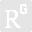
\includegraphics[width=1em]{img/RG-dark.png}~}

 \begin{document}
 \pagecolor{backgroundcolor}
% ---

% HEADING
\begin{tabular*}{\textwidth}{l@{\extracolsep{\fill}}r}
  \textbf{\href{https://www.pedrolarben.com}{\LARGE Pedro Lara-Benítez}} &  \\
  {{\Large Machine Learning Researcher}} &  \href{https://github.com/pedrolarben}{ \faicon{github} \color{urlcolor} pedrolarben} \\
  \href{mailto:pedrolarabenitez@gmail.com}{pedrolarabenitez@gmail.com} &  \href{https://www.linkedin.com/in/pedrolarben }{ \faicon{linkedin} \color{urlcolor} }  \href{https://scholar.google.com/citations?user=vrWKUgcAAAAJ&hl }{ \faicon{graduation-cap} \color{urlcolor} } 
  \href{https://www.researchgate.net/profile/Pedro_Lara-Benitez }{ \researchgatesocialsymbol \color{urlcolor} } \\
  \href{tel:+447895284760}{07895 284760} \hspace{0.5em} London, UK &  \faicon{code} Python, Java, C, R\\
  \textsl{\small \latestVersion} & \textsl{\small \otherThemeRef}
\end{tabular*}
% ---
\vspace{-2em}
\section*{}
\justifying
% Research-focused professional with strong programming and mathematical skills in algebra and statistics. Hands-on experience providing valuable insights via data analytics and advanced data-driven methods. Proven success developing high quality code with detailed documentation to support reproducible research. Passionate about core machine learning principles, data sciences, deep learning, engineering, and research. Track record of conducting cutting-edge research on distributed artificial intelligence to develop state-of-the-art solutions for real-world problems.
Research-focused quantitative professional combining deep technical expertise in machine learning with practical financial industry experience. Track record of developing innovative solutions in distributed computing, risk analytics, and artificial intelligence, with multiple peer-reviewed publications in leading journals.

% EXPERIENCE
\section{Experience}
  \resumeSubHeadingListStart
    \resumeSubheading{Bank of America}{London, UK}
      {Vice President (VP) - Quantitative Financial Analyst}{February 2024 - Present} 
      \resumeItemListStart  
        \resumeItem{Architected and implemented a distributed computing framework for model analysis, enabling efficient model calculations, including full-revaluation and risk-theoretical P\&L, under the FRTB regulatory framework.} 
        \resumeItem{Developed interactive dashboards for framework monitoring and control, improving user experience and operational visibility.} 
        \resumeItem{Built an automated big-data analytics pipeline for VaR accuracy and P\&L attribution analysis, delivering actionable risk insights.} 
      \resumeItemListEnd
          
    \resumeSubSubheading 
      {Assistant Vice President (AVP) - Quantitative Financial Analyst}{May 2022 - January 2024} 
      \resumeItemListStart 
        \resumeItem{Led development of Risk Not in Stress (RNiS) application, transforming manual spreadsheet processes into an automated web-based solution.} 
        \resumeItem{Contributed to critical risk processes including VaR Backtesting and Overage Explains, improving operational efficiency.} 
        \resumeItem{Collaborated with cross-functional teams to align project goals and ensure seamless execution and handoffs.} 
      \resumeItemListEnd
          
    \resumeSubSubheading {Contractor - Quantitative Developer}{May 2021 - May 2022} 
      \resumeItemListStart 
        \resumeItem{Enhanced Risk Not in VaR (RNiV) Calculator using React/Python, implementing robust testing and code review practices in an agile environment.} 
      \resumeItemListEnd

    \resumeTech{Team}{Process Engineering, Global Risk Analytics - Financial data analysis and software development}

    \resumeSubheading{University of Seville}{Seville, Spain}
      {Machine Learning Researcher}{October 2018 - May 2021}
      \resumeItemListStart
        \resumeItem{Carry out experiments regarding deep learning, interpret results, and produce a written paper with conclusions of study.}
        \resumeItem{Demonstrate expertise in the state-of-art techniques of the field.}
        \resumeItem{Reviewed and published research papers in top-tier peer-reviewed journals and international conferences.}
      \resumeItemListEnd
      \resumeTech{Technologies}{python, tensorflow, keras, pytorch, numpy, sci-kit, matplotlib, latex, AWS.}\\
      \resumeTech{Theory}{Deep Learning, Time series forecasting, Online learning, Data stream, and Computer vision.}

    \resumeSubheading{\textit{Additional Experience}}{Seville, Spain}
      {Freelance Software Developer}{2017 - 2019}
      \resumeItemListStart
        \resumeItem{Android App for MSIG Smart Management and web information system for BBA Medical Centre.}
      \resumeItemListEnd

  \resumeSubHeadingListEnd
% ---
% PROGRAMMING SKILLS
\section{Technical Proficiencies}
  \resumeSubHeadingListStart
  
  \resumeSubItem{\textbf{Programming Languages:} Python, JavaScript, Java, SQL}
  
  \resumeSubItem{\textbf{ML/AI Frameworks:} TensorFlow, PyTorch, scikit-learn, XGBoost}
  
  \resumeSubItem{\textbf{Data Processing \& Analytics:} Pandas, NumPy, River, DuckDB, Pyarrow, Plotly, Matplotlib, Dash}
  
  \resumeSubItem{\textbf{Web Development:} React, Vue, Flask, Django, RESTful APIs}
  
  \resumeSubItem{\textbf{Infrastructure:} AWS, Azure, Docker, Git, Linux, Distributed Computing}
  
  \resumeSubItem{\textbf{Domain Expertise:} Deep Learning, Time Series Analysis, Risk Analytics, FRTB, VaR, P\&L Attribution}
  
  \resumeSubHeadingListEnd

% EDUCATION
\section{Education}
  \resumeSubHeadingListStart
    \resumeSubheading
      {University of Seville}{Seville, Spain}
      {PhD in Computer Science - Machine Learning }{Sept. 2019 -- July 2022}
      \resumeItemListStart
      \resumeItem{Researched about data science, machine learning and artificial intelligence. Mainly focused on deep learning, time series analysis, online learning and object detection.}
      \resumeItemListEnd
      \resumeTech{Thesis}{Online Streaming Time Series Forecasting with Deep Learning.}
    \resumeSubheading
      {University of Seville}{Seville, Spain}
      {M.Sc in Software Engineering: Cloud, Data Science \& IT Service Management - 9.26/10}{Sept. 2018 -- Jun. 2019}
      \resumeItemListStart
      \resumeItem{Took selective courses on: Data Engineering, Machine Learning, Data visualisation techniques, Analysis of unstructured information, Big Data, Data Science.}
      \resumeItem{(Thesis title) Asynchronous framework for the application of Deep Learning to streaming data.}
      \resumeItemListEnd
    \resumeSubheading
      {Middlesex University}{London, UK}
      {[Erasmus year abroad] B.Sc in Computer Science}{Sept. 2017 -- Jun. 2018}
      \resumeItemListStart
      \resumeItem{Took selective courses on: Open Source Software, Quantum Information Theory and Artificial Intelligence.}
      \resumeItemListEnd
    \resumeSubheading
      {University of Seville}{Seville, Spain}
      {B.Sc in Computer Science - Software Engineering - 8.55/10}{Sept. 2014 -- Jun. 2018}
      \resumeItemListStart
      \resumeItem{Took courses such as: Statistics, Analysis and Design of Data structures and Algorithms, or Artificial Intelligence.}
      \resumeItem{(Thesis title) Biomedical data analysis with deep learning.}
      \resumeItemListEnd
  \resumeSubHeadingListEnd
% ---

\hfill \textsl{ \faicon{link}Following sections items are clickable for references.}
\vspace{-1.5em}

% CERTIFICATIONS
%\section{Certifications}
%  \resumeSubHeadingListStart
%    \resumeSubheading
%      {Coursera}{MOOC}
%      {\href{https://www.coursera.org/account/accomplishments/specialization/certificate/WYGXVXA327K9}{Deep learning Specialization}}{Issued January 2021}
%    
%    \resumeSubSubheading
%     {\href{https://www.coursera.org/account/accomplishments/verify/HEURLGHTW46G}{Sequence Models}}{Issued January 2021}
%      
%    \resumeSubSubheading
%     {\href{https://www.coursera.org/account/accomplishments/verify/U59ZPPWP5NRN}{Convolutional Neural Networks}}{Issued September 2020}
%    
%    \resumeSubSubheading
%     {\href{https://www.coursera.org/account/accomplishments/verify/BHN34W5WKBUT}{Structuring Machine Learning Projects}}{Issued May 2020} 
%   
%    \resumeSubSubheading
%     {\href{https://www.coursera.org/account/accomplishments/records/J76SQGG4PVYL}{Improving Deep Neural Networks: Hyperparameter tuning, Regularization and %Optimization}}{Issued May 2020}
%     
%    \resumeSubSubheading
%     {\href{https://www.coursera.org/account/accomplishments/verify/MBWJ69CVLQAZ}{Neural Networks and Deep Learning}}{Issued May 2020}
%      
%    \resumeSubSubheading
%     {\href{https://www.coursera.org/account/accomplishments/certificate/MZ7TC7ADV7YY}{R Programming}}{Issued September 2016}
%      
%    \resumeSubSubheading
%     {\href{https://www.coursera.org/account/accomplishments/certificate/36JC577GBFYD}{Text Mining and Analytics}}{Issued August 2016}
%     
%    \resumeSubSubheading
%     {\href{https://www.coursera.org/account/accomplishments/certificate/MDWATFKLPH9Z}{Text retrieval and search engines}}{Issued June 2016}
%     
%    \resumeSubSubheading
%     {\href{https://www.coursera.org/account/accomplishments/certificate/TM7T8CJXNV6R}{The Data Scientist's Toolbox}}{Issued June 2016}
%     
%    \resumeSubSubheading
%     {\href{https://www.coursera.org/account/accomplishments/certificate/WYGG7TDFPB3F}{Data Visualization}}{Issued March 2016}
%  \resumeSubHeadingListEnd
% ---

%\newpage



% RESEARCH PUBLICATIONS
\section{Research publications}

  \resumeSubHeadingListStart
    \resumeSubItem{\href{https://doi.org/10.1016/j.ijepes.2023.109730}{Riquelme-Dominguez, J. M., Carranza-García, M., Lara-Benítez, P., and González-Longatt, F. M. "\textbf{A machine learning-based methodology for short-term kinetic energy forecasting with real-time application: Nordic Power System case.}" International Journal of Electrical Power \& Energy Systems, vol. 156, p. 109730, DOI:10.1016/j.ijepes.2023.109730, Feb 2024.}}
  
    \resumeSubItem{\href{https://doi.org/10.1016/j.neucom.2023.126312}{Lara-Benítez, P., Carranza-García, M., Luna-Romera, J. M., and Riquelme, J. C. "\textbf{Short-term solar irradiance forecasting in streaming with deep learning.}" Neurocomputing, vol. 546, p. 126312, DOI:10.1016/j.neucom.2023.126312, Aug 2023.}}
  
    \resumeSubItem{\href{https://doi.org/10.1093/jigpal/jzac033}{Lara-Benítez, P., Carranza-García, M., Gutiérrez-Avilés, D., and Riquelme, J. C. "\textbf{Data streams classification using deep learning under different speeds and drifts.}" Logic Journal of the IGPL, DOI:10.1093/jigpal/jzac033, Feb 2022.}}

    \resumeSubItem{\href{https://doi.org/10.1007/978-3-030-85713-4_11}{Lara-Benítez, P., Gallego-Ledesma, L., Carranza-García, M., and Luna-Romera, J. M. "\textbf{Evaluation of the Transformer Architecture for Univariate Time Series Forecasting.}" XIX Conference of the Spanish Association for Artificial Intelligence (CAEPIA), pp. 106-115, Springer, DOI:10.1007/978-3-030-85713-4\_11, May 2021.}}
  
    \resumeSubItem{\href{https://doi.org/10.1007/978-3-030-87869-6_62}{Carranza-García, M.,  Lara-Benítez, P., and Riquelme, J. C. "\textbf{Feature selection on spatio-temporal data for solar irradiance forecasting.}" \nth{16} International Conference on Soft Computing Models in Industrial and Environmental Applications (SOCO 21), pp. 654-664, Springer, DOI:10.1007/978-3-030-87869-6\_62 May 2021.}}
    
    \resumeSubItem{\href{https://arxiv.org/abs/2104.03888}{Carranza-García, M.,  Lara-Benítez, P., García-Gutiérrez, J., and Riquelme, J. C. "\textbf{Enhancing Object Detection in Autonomous Vehicles by Optimizing Anchor Generation and Addressing Class Imbalance.}" Neurocomputing, vol 449, p. 229-244, DOI:10.1016/j.neucom.2021.04.001, Apr 2021.}}
    
    \resumeSubItem{\href{https://arxiv.org/abs/2103.12057}{Lara-Benítez, P., Carranza-García, M., and Riquelme, J. C. "\textbf{An Experimental Review on Deep Learning Architectures for Time Series Forecasting.}" International Journal of Neural Systems, vol. 31, no 03. p. 2130001, DOI:10.1142/S0129065721300 011, Feb 2021.}}
    
    \resumeSubItem{\href{https://doi.org/10.3390/rs13010089}{Carranza-García, M., Torres-Mateo, J., Lara-Benítez, P., and García-Gutiérrez, J. "\textbf{On the performance of one-stage and two-stage object detectors in autonomous vehicles using camera data.}" Remote Sensing, vol. 13, no 1, p. 89, DOI:10.3390/rs13010089, Nov 2020.}}
    
    \resumeSubItem{\href{https://doi.org/10.1007/978-3-030-57802-2_14}{Lara-Benítez, P., Carranza-García, M., Martínez-Álvarez, F, and Riquelme, J. C. "\textbf{On the performance of deep learning models for time series classification in streaming.}" 15th International Conference on Soft Computing Models in Industrial and Environmental Applications (SOCO 2020), vol. 1268, pp 144-154, Springer International Publishing, DOI:10.1007/978-3-030-57802-2\_14, Aug 2020.}}
    
    \resumeSubItem{\href{https://doi.org/10.3390/app10072322}{Lara-Benítez, P., Carranza-García, M., Luna-Romera, J. M., Riquelme, J. C. "\textbf{Temporal Convolutional Networks Applied to Energy-Related Time Series Forecasting." Applied Sciences.} , vol. 10, pp 2322, DOI:10.3390/app10072322, March 2020.}}
    
    \resumeSubItem{\href{https://www.researchgate.net/publication/338590631_Asynchronous_dual-pipeline_deep_learning_framework_for_online_data_stream_classification}{Lara-Benítez, P., Carranza-García, M., García-Gutiérrez, J., and Riquelme, J. C. "\textbf{Asynchronous dual-pipeline deep learning framework for online data stream classification.}" Integrated Computer-Aided Engineering, vol. 27, no. 2, pp. 101-119, DOI:10.3233/ICA-200617, Feb 2020.}}

    
  \resumeSubHeadingListEnd
% ---

% PROJECTS
\section{Personal Projects}

  \resumeSubHeadingListStart
    \resumeSubItem{\href{https://adlstream.readthedocs.io/}{ADLStream: A python open source library for online learning with Deep Learning models.}}

    \resumeSubItem{\href{https://github.com/tensorflow/addons/pull/1811/files}{Contribution to TensorFlow Addons with Echo State Network (ESN) implementation.}}
    
  \resumeSubHeadingListEnd
% ---

\vspace{-0.5em}
\hfill \textsl{ Not clickable anymore.}
\vspace{-1.5em}

%Awards
\section{Awards}
  \resumeSubHeadingListStart
      \resumeSubheadingTwo{Winner of "Atmira Stock Prediction" challenge in the UniversityHack 2021 Datathon,}{the largest data analysis competition in Spain.}{2021}
      {Cajamar Data Lab}{}
      \vspace{-0.5em}
      
      \resumeSubheadingTwo{Selected as one of the top 30 computer-science pre-doctoral student nationwide for}{a 4-year research fellowship (FPU). }{2020}
      {Ministry of Science, Innovation and Universities; Government of Spain.}{}
      \vspace{-0.5em}
      
      \resumeSubheading{Winner of OpenWebnars' Prize and \nth{2} Prize in Start-up Hackathon "Hack for good".}{2017}
      {Think Big, Fundación Telefónica}{}
      \vspace{-0.5em}

      \resumeSubheading{Finalist Circular Economy Start-up contest.}{2016}
      {GO APP! by Google}{}
      \vspace{-0.5em}

      \resumeSubheading{\nth{1} Prize in Code Competition "Everis Codefest Sevilla".}{2016}
      {Everis}{}
  
  \resumeSubHeadingListEnd

%LANGUAGES
\section{Languages}
  \resumeSubHeadingListStart
  
  \resumeSubItem{\textbf{Spanish} (Native), \textbf{English} (C1 Advanced), \textbf{Italian} (B1 Basic) }
  
  \resumeSubHeadingListEnd


% ---
\end{document}
